% Options for packages loaded elsewhere
\PassOptionsToPackage{unicode}{hyperref}
\PassOptionsToPackage{hyphens}{url}
%
\documentclass[
  letterpaper,
  ignorenonframetext,
  aspectratio=43,
  handout,
  12pt]{beamer}
\usepackage{pgfpages}
\setbeamertemplate{caption}[numbered]
\setbeamertemplate{caption label separator}{: }
\setbeamercolor{caption name}{fg=normal text.fg}
\beamertemplatenavigationsymbolsempty
% Prevent slide breaks in the middle of a paragraph
\widowpenalties 1 10000
\raggedbottom
\setbeamertemplate{part page}{
  \centering
  \begin{beamercolorbox}[sep=16pt,center]{part title}
    \usebeamerfont{part title}\insertpart\par
  \end{beamercolorbox}
}
\setbeamertemplate{section page}{
  \centering
  \begin{beamercolorbox}[sep=12pt,center]{part title}
    \usebeamerfont{section title}\insertsection\par
  \end{beamercolorbox}
}
\setbeamertemplate{subsection page}{
  \centering
  \begin{beamercolorbox}[sep=8pt,center]{part title}
    \usebeamerfont{subsection title}\insertsubsection\par
  \end{beamercolorbox}
}
\AtBeginPart{
  \frame{\partpage}
}
\AtBeginSection{
  \ifbibliography
  \else
    \frame{\sectionpage}
  \fi
}
\AtBeginSubsection{
  \frame{\subsectionpage}
}
\usepackage{amsmath,amssymb}
\usepackage{lmodern}
\usepackage{ifxetex,ifluatex}
\ifnum 0\ifxetex 1\fi\ifluatex 1\fi=0 % if pdftex
  \usepackage[T1]{fontenc}
  \usepackage[utf8]{inputenc}
  \usepackage{textcomp} % provide euro and other symbols
\else % if luatex or xetex
  \usepackage{unicode-math}
  \defaultfontfeatures{Scale=MatchLowercase}
  \defaultfontfeatures[\rmfamily]{Ligatures=TeX,Scale=1}
\fi
\usetheme[]{metropolis}
% Use upquote if available, for straight quotes in verbatim environments
\IfFileExists{upquote.sty}{\usepackage{upquote}}{}
\IfFileExists{microtype.sty}{% use microtype if available
  \usepackage[]{microtype}
  \UseMicrotypeSet[protrusion]{basicmath} % disable protrusion for tt fonts
}{}
\makeatletter
\@ifundefined{KOMAClassName}{% if non-KOMA class
  \IfFileExists{parskip.sty}{%
    \usepackage{parskip}
  }{% else
    \setlength{\parindent}{0pt}
    \setlength{\parskip}{6pt plus 2pt minus 1pt}}
}{% if KOMA class
  \KOMAoptions{parskip=half}}
\makeatother
\usepackage{xcolor}
\IfFileExists{xurl.sty}{\usepackage{xurl}}{} % add URL line breaks if available
\IfFileExists{bookmark.sty}{\usepackage{bookmark}}{\usepackage{hyperref}}
\hypersetup{
  hidelinks,
  pdfcreator={LaTeX via pandoc}}
\urlstyle{same} % disable monospaced font for URLs
\newif\ifbibliography
\usepackage{graphicx}
\makeatletter
\def\maxwidth{\ifdim\Gin@nat@width>\linewidth\linewidth\else\Gin@nat@width\fi}
\def\maxheight{\ifdim\Gin@nat@height>\textheight\textheight\else\Gin@nat@height\fi}
\makeatother
% Scale images if necessary, so that they will not overflow the page
% margins by default, and it is still possible to overwrite the defaults
% using explicit options in \includegraphics[width, height, ...]{}
\setkeys{Gin}{width=\maxwidth,height=\maxheight,keepaspectratio}
% Set default figure placement to htbp
\makeatletter
\def\fps@figure{htbp}
\makeatother
% Make links footnotes instead of hotlinks:
\DeclareRobustCommand{\href}[2]{#2\footnote{\url{#1}}}
\setlength{\emergencystretch}{3em} % prevent overfull lines
\providecommand{\tightlist}{%
  \setlength{\itemsep}{0pt}\setlength{\parskip}{0pt}}
\setcounter{secnumdepth}{-\maxdimen} % remove section numbering
\usepackage{pgfpages}
\pgfpagesuselayout{2 on 1}
\providecommand{\tightlist}{%
\setlength{\itemsep}{0pt}\setlength{\parskip}{0pt}}
\makeatletter
\makeatother
\let\Oldincludegraphics\includegraphics
\renewcommand{\includegraphics}[2][]{\Oldincludegraphics[width=\textwidth,height=0.7\textheight,keepaspectratio]{#2}}
\ifluatex
  \usepackage{selnolig}  % disable illegal ligatures
\fi

\author{}
\date{}

\begin{document}

\begin{frame}{AE 737: Mechanics of Damage Tolerance}
\protect\hypertarget{ae-737-mechanics-of-damage-tolerance}{}
Lecture 6 - Plastic Zone

Dr.~Nicholas Smith

Wichita State University, Department of Aerospace Engineering

February 17, 2021
\end{frame}

\begin{frame}{schedule}
\protect\hypertarget{schedule}{}
\begin{itemize}
\tightlist
\item
  17 Feb - Plastic Zone, HW 2 Due, HW 1 Self-grade due
\item
  22 Feb - Fracture Toughness
\item
  24 Feb - Fracture Toughness, HW3 Due, HW 2 Self-grade due
\item
  1 Mar - Residual Strength
\end{itemize}
\end{frame}

\begin{frame}{outline}
\protect\hypertarget{outline}{}
\begin{itemize}
\tightlist
\item
  plastic zone
\item
  plastic stress intensity ratio
\item
  plastic zone shape
\item
  group problems
\end{itemize}
\end{frame}

\hypertarget{plastic-zone}{%
\section{plastic zone}\label{plastic-zone}}

\begin{frame}{plastic zone}
\protect\hypertarget{plastic-zone-1}{}
\begin{itemize}
\tightlist
\item
  Previous developments assumed perfectly elastic materials
\item
  Most common materials have some plasticity
\item
  Any stress above the yield stress will undergo plastic deformation (no
  stress higher than \(\sigma_y\) will be present in the material)
\end{itemize}
\end{frame}

\begin{frame}{plastic zone}
\protect\hypertarget{plastic-zone-2}{}
\begin{itemize}
\tightlist
\item
  Plasticity helps retard crack propagation due to residual stresses
\item
  After an overload, elastic regions will contract back to their
  undeformed shape
\item
  The region which has undergone plastic deformation, however, holds its
  deformed shape
\item
  This introduces a region of residual compressive stress near the crack
  tip
\item
  Before the crack can propagate, a stress needs to overcome this
  residual stress
\end{itemize}
\end{frame}

\begin{frame}{2D problems}
\protect\hypertarget{d-problems}{}
\begin{itemize}
\tightlist
\item
  We often simplify the full 3D elasticity equations for planar problems
\item
  For very thin panels, we assume that all out-of-plane stresses are 0
\item
  This is called plane stress
\end{itemize}
\end{frame}

\begin{frame}{plane stress}
\protect\hypertarget{plane-stress}{}
\[\begin{aligned}
  \sigma_z &= \tau_{xz} = \tau_{zy} = 0\\
  \epsilon_x &= \frac{\sigma_x}{E} - \nu \frac{\sigma_y}{E}\\
  \epsilon_y &= -\nu \frac{\sigma_x}{E} + \frac{\sigma_y}{E}\\
  \epsilon_z &= -\nu \frac{\sigma_x}{E} - \nu \frac{\sigma_y}{E}\\
  \gamma_{xy} &= \frac{\tau_{xy}}{G}\\
  \gamma_{xz} &= \gamma_{yz} = 0
\end{aligned}\]
\end{frame}

\begin{frame}{2D problems}
\protect\hypertarget{d-problems-1}{}
\begin{itemize}
\tightlist
\item
  When instead a panel is very thick, we assume that any strains through
  the thickness are small relative to other strains
\item
  \(\epsilon_z = \gamma_{xz} = \gamma_{yz} = 0\)
\item
  This is known as plane strain
\end{itemize}
\end{frame}

\begin{frame}{plane strain}
\protect\hypertarget{plane-strain}{}
\[\begin{aligned}
  \epsilon_x &= \frac{\sigma_x}{E} - \nu \frac{\sigma_y}{E} - \nu \frac{\sigma_z}{E}\\
  \epsilon_y &= -\nu \frac{\sigma_x}{E} + \frac{\sigma_y}{E} - \nu \frac{\sigma_z}{E}\\
  0 &= -\nu \frac{\sigma_x}{E} - \nu \frac{\sigma_y}{E} + \frac{\sigma_z}{E}\\
  \gamma_{xy} &= \frac{\tau_{xy}}{G}\\
  \gamma_{xz} &= \gamma_{yz} = 0
\end{aligned}\]
\end{frame}

\begin{frame}{Irwin's first approximation}
\protect\hypertarget{irwins-first-approximation}{}
\begin{itemize}
\tightlist
\item
  If we recall the equation for opening stress (\(\sigma_y\)) near the
  crack tip
\end{itemize}

\[\sigma_y = \frac{K_I}{\sqrt{2\pi r}} \cos \frac{\theta}{2} \left(1+\sin \frac{\theta}{2}\sin \frac{3\theta}{2}\right) \tag{1.2}\]

\begin{itemize}
\tightlist
\item
  In the plane of the crack, when \(\theta=0\) we find
\end{itemize}

\[\sigma_y = \frac{K_I}{\sqrt{2\pi r}}\]
\end{frame}

\begin{frame}{Irwin's first approximation}
\protect\hypertarget{irwins-first-approximation-1}{}
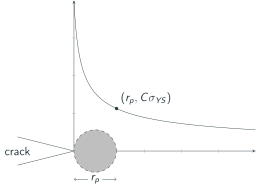
\includegraphics{../images/plastic-zone.svg}
\end{frame}

\begin{frame}{Irwin's first approximation}
\protect\hypertarget{irwins-first-approximation-2}{}
\begin{columns}[T]
\begin{column}{0.5\textwidth}
\begin{itemize}
\tightlist
\item
  We use \emph{C}, the \emph{Plastic Constraint Factor} to convert
  between Plane Strain and Plane Stress solutions
\item
  The plastic zone size can now be approximated
\end{itemize}
\end{column}

\begin{column}{0.5\textwidth}
\[\begin{aligned}
  \sigma_{yy}(r=r_p) &= C\sigma_{YS}\\
  \frac{K_I}{\sqrt{2\pi r_p}} &= C\sigma_{YS}\\
  r_p &= \frac{1}{2\pi} \left(\frac{K_I}{C\sigma_{YS}}\right)^2
\end{aligned}\]
\end{column}
\end{columns}
\end{frame}

\begin{frame}{Irwin's first approximation}
\protect\hypertarget{irwins-first-approximation-3}{}
\begin{itemize}
\tightlist
\item
  For plane stress (thin panels) we let \(C=1\) and find
  \emph{r}\emph{p} as
\end{itemize}

\[r_p = \frac{1}{2\pi} \left(\frac{K_I}{\sigma_{YS}}\right)^2\]

\begin{itemize}
\tightlist
\item
  And for plane strain (thick panels) we let \(C=\sqrt{3}\) and find
\end{itemize}

\[r_p = \frac{1}{6\pi} \left(\frac{K_I}{\sigma_{YS}}\right)^2\]
\end{frame}

\begin{frame}{Intermediate panels}
\protect\hypertarget{intermediate-panels}{}
\begin{itemize}
\tightlist
\item
  For panels which lie between plane strain and plane stress states, we
  use the following expression to estimate the plastic zone size
\end{itemize}

\[r_p = \frac{1}{I\pi} \left(\frac{K_I}{\sigma_{YS}}\right)^2\]

\begin{itemize}
\tightlist
\item
  Where \emph{I} is defined as
\end{itemize}

\[I = 6.7 - \frac{1.5}{t}\left(\frac{K_I}{\sigma_{YS}}\right)^2\]

\begin{itemize}
\tightlist
\item
  And \(2 \le I \le 6\)
\end{itemize}
\end{frame}

\begin{frame}{Irwin's second approximation}
\protect\hypertarget{irwins-second-approximation}{}
\begin{itemize}
\tightlist
\item
  If our material is perfectly elastic-plastic, no stresses above
  \(C\sigma_{ys}\) will exist in the material
\item
  This ignores the strain energy (represented by the area under the
  curve) in the plastic zone
\end{itemize}
\end{frame}

\begin{frame}{Irwin's second approximation}
\protect\hypertarget{irwins-second-approximation-1}{}
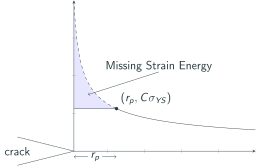
\includegraphics{../images/plastic-missing.svg}
\end{frame}

\begin{frame}{Irwin's second approximation}
\protect\hypertarget{irwins-second-approximation-2}{}
\begin{itemize}
\tightlist
\item
  To account for the additional strain energy, Irwin considered a
  plastic zone size increased by some \$\delta\$
\item
  He also needed to adjust the stress function, and considered an
  equivalent crack tip in these calculations
\end{itemize}
\end{frame}

\begin{frame}{Irwin's second approximation}
\protect\hypertarget{irwins-second-approximation-3}{}
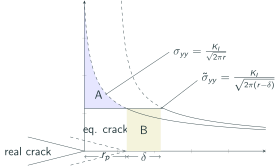
\includegraphics{../images/plastic-equivalent.svg}
\end{frame}

\begin{frame}{Irwin's second approximation}
\protect\hypertarget{irwins-second-approximation-4}{}
\begin{columns}[T]
\begin{column}{0.5\textwidth}
We need \emph{A}=\emph{B}, so we set them equivalent and solve for
\(\delta\).
\end{column}

\begin{column}{0.5\textwidth}
\[\begin{aligned}
  A &= \int_{0}^{r_p} \sigma_{yy} dr - r_p \sigma_{YS}\\
  &= \int_{0}^{r_p} \frac{K_I}{\sqrt{2\pi r}} dr - r_p \sigma_{YS}\\
  &= \frac{K_I}{\sqrt{2\pi}}\int_{0}^{r_p} r^{-1/2} dr - r_p \sigma_{YS}\\
  &= \frac{2K_I \sqrt{r_p}}{\sqrt{2\pi}}- r_p \sigma_{YS}
\end{aligned}\]
\end{column}
\end{columns}
\end{frame}

\begin{frame}{Irwin's second approximation}
\protect\hypertarget{irwins-second-approximation-5}{}
\begin{itemize}
\tightlist
\item
  We have already found \emph{r}\emph{p} as
\end{itemize}

\[r_p = \frac{1}{2\pi} \left(\frac{K_I}{\sigma_{YS}}\right)^2\]

\begin{itemize}
\tightlist
\item
  If we solve this for \emph{K}\emph{I} we find
\end{itemize}

\[K_I = \sqrt{2\pi r_p} \sigma_{YS}\]
\end{frame}

\begin{frame}{Irwin's second approximation}
\protect\hypertarget{irwins-second-approximation-6}{}
\begin{itemize}
\tightlist
\item
  We can now substitute back into the strain energy of A
\end{itemize}

\[\begin{aligned}
  A &= \frac{2\sqrt{2\pi r_p} \sigma_{YS} \sqrt{r_p}}{\sqrt{2\pi}}- r_p \sigma_{YS}\\
  &= 2 \sigma_{YS} r_p- r_p \sigma_{YS}\\
  &= r_p \sigma_{YS}
\end{aligned}\]
\end{frame}

\begin{frame}{Irwin's second approximation}
\protect\hypertarget{irwins-second-approximation-7}{}
\begin{itemize}
\tightlist
\item
  B is given simply as \(B=\delta \sigma_{ys}\) so we equate A and B to
  find \$\delta\$
\end{itemize}

\[\begin{aligned}
  A &= B\\
  r_p \sigma_{YS} &= \delta \sigma_{YS}\\
  r_p &= \delta
\end{aligned}\]
\end{frame}

\begin{frame}{Irwin's second approximation}
\protect\hypertarget{irwins-second-approximation-8}{}
\begin{itemize}
\tightlist
\item
  This means the plastic zone size is simply 2\emph{r}\emph{p}
\item
  However, it also means that the effective crack length is
  \emph{a}+\emph{r}\emph{p}
\item
  Since \emph{r}\emph{p} depends on \emph{K}\emph{I}, we must iterate a
  bit to find the ``real'' \emph{r}\emph{p} and \emph{K}\emph{I}
\end{itemize}
\end{frame}

\begin{frame}{Example}
\protect\hypertarget{example}{}
\begin{figure}
\centering
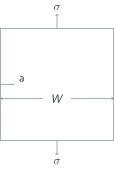
\includegraphics{../images/plastic-example.svg}
\caption{An edge crack of length a in a panel of width W is subjected to
a remote load}
\end{figure}
\end{frame}

\begin{frame}{equations}
\protect\hypertarget{equations}{}
\[\begin{aligned}
  \beta &= \left[1.122 - 0.231 \frac{a}{W} + 10.55 \left(\frac{a}{W}\right)^2 - 21.71 \left(\frac{a}{W}\right)^3 + 30.82 \left(\frac{a}{W}\right)^4\right] \\
  I &= 6.7 - \frac{1.5}{t}\left(\frac{K_I}{\sigma_{YS}}\right)^2 \\
  r_p &= \frac{1}{I\pi} \left(\frac{K_I}{\sigma_{YS}}\right)^2
\end{aligned}\] \href{../examples/Plastic\%20Zone\%20Example.html}{work}
\end{frame}

\hypertarget{plastic-stress-intensity-ratio}{%
\section{plastic stress intensity
ratio}\label{plastic-stress-intensity-ratio}}

\begin{frame}{plastic stress intensity ratio}
\protect\hypertarget{plastic-stress-intensity-ratio-1}{}
\begin{itemize}
\tightlist
\item
  Engineers often use stress intensity to decide which material to use
  for a certain application
\item
  The ratio of plastic stress intensity to elastic stress intensity, as
  a function of yield stress over applied stress, can help illustrate
  the effects of plasticity for different materials.
\end{itemize}
\end{frame}

\begin{frame}{plastic stress intensity ratio}
\protect\hypertarget{plastic-stress-intensity-ratio-2}{}
\begin{columns}[T]
\begin{column}{0.5\textwidth}
For an infinitely wide center-cracked panel, we can solve for
\emph{K}\emph{Ie}/\emph{K}\emph{I} symbolically, in plane stress
\end{column}

\begin{column}{0.5\textwidth}
\[\begin{aligned}
  K_I &= \sigma \sqrt{\pi a}\\
  K_{Ie} &= \sigma \sqrt{\pi(a+r_p)}\\
  r_p &= \frac{1}{2\pi} \left( \frac{K_{Ie}}{\sigma_{YS}}\right)^2\\
  K_{Ie} &= \sigma \sqrt{\pi \left(a+\frac{1}{2\pi} \left( \frac{K_{Ie}}{\sigma_{YS}}\right)^2\right)}
\end{aligned}\]
\end{column}
\end{columns}
\end{frame}

\begin{frame}{stress intensity ratio}
\protect\hypertarget{stress-intensity-ratio}{}
\[\begin{aligned}
  K_{Ie}^2 &= \sigma^2 \pi \left(a+\frac{1}{2\pi} \left( \frac{K_{Ie}}{\sigma_{YS}}\right)^2\right)\\
  K_{Ie}^2 &= \sigma^2 \pi a+\frac{\sigma^2}{2} \left( \frac{K_{Ie}}{\sigma_{YS}}\right)^2\\
  K_{Ie}^2 - \frac{\sigma^2}{2} \left( \frac{K_{Ie}}{\sigma_{YS}}\right)^2 &= \sigma^2 \pi a\\
  K_{Ie}^2\left(1 - \frac{\sigma^2}{2 \sigma_{YS}^2}\right) &= \sigma^2 \pi a
\end{aligned}\]

Note: square both sides
\end{frame}

\begin{frame}{plastic stress intensity ratio}
\protect\hypertarget{plastic-stress-intensity-ratio-3}{}
\[\begin{aligned}
  K_{Ie}^2 &= \frac{\sigma^2 \pi a}{1 - \frac{\sigma^2}{2 \sigma_{YS}^2}}\\
  K_{Ie} &= \frac{\sigma \sqrt{\pi a}}{\sqrt{1 - \frac{\sigma^2}{2 \sigma_{YS}^2}}}\\
  K_{Ie} &= \frac{K_I}{\sqrt{1 - \frac{\sigma^2}{2 \sigma_{YS}^2}}}\\
  \frac{K_{Ie}}{K_I} &= \frac{1}{\sqrt{1 - \frac{\sigma^2}{2 \sigma_{YS}^2}}}
\end{aligned}\]

Note: We divide both sides by
\(\left(1 - \frac{\sigma^2}{2 \sigma_{YS}^2}\right)\)
\end{frame}

\begin{frame}{plastic stress intensity ratio}
\protect\hypertarget{plastic-stress-intensity-ratio-4}{}
\begin{itemize}
\tightlist
\item
  We can also find the plastic stress intensity ratio numerically for
  finite width panels
\item
  Panel thickness, yield stress, panel width, crack length could all be
  variables in this case
\item
  Different heat treatments of metal alloys can give a different yield
  stress, with most other properties remaining the same
\item
  Typical crack lengths can vary based on inspection cycles
\end{itemize}
\end{frame}

\begin{frame}{example}
\protect\hypertarget{example-1}{}
\begin{columns}[T]
\begin{column}{0.5\textwidth}
\begin{itemize}
\tightlist
\item
  You are asked to design an inspection cycle for a panel
\item
  Consider the plastic stress intensity ratio, and the effect of varying
  crack lengths on it
\end{itemize}
\end{column}

\begin{column}{0.5\textwidth}
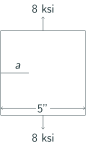
\includegraphics{../images/intensity-ratio-example.svg}
\end{column}
\end{columns}
\end{frame}

\begin{frame}{example}
\protect\hypertarget{example-2}{}
online example
\href{../examples/Plastic\%20stress\%20intensity\%20ratio.html}{here}
\end{frame}

\hypertarget{plastic-zone-shape}{%
\section{plastic zone shape}\label{plastic-zone-shape}}

\begin{frame}{plastic zone shape}
\protect\hypertarget{plastic-zone-shape-1}{}
\begin{itemize}
\tightlist
\item
  Although we drew a circle to give a rough idea of the plastic zone in
  Irwin's method, this solution was only 1D
\item
  We considered \(\theta=0\).
\item
  It is advantageous to model the plastic zone shape, we will do so
  using two different yield theories
\item
  Von Mises and Tresca
\end{itemize}
\end{frame}

\begin{frame}{principal stresses}
\protect\hypertarget{principal-stresses}{}
\begin{itemize}
\tightlist
\item
  Principal stresses are often used in yield theories
\item
  We can determine the principal stresses near the crack tip as
\end{itemize}

\[\begin{aligned}
  \label{eq:principal}
  \sigma_1 &= \frac{K_I}{\sqrt{2\pi r}}\cos \frac{\theta}{2}\left(1+\sin \frac{\theta}{2}\right)&\\
  \sigma_2 &= \frac{K_I}{\sqrt{2\pi r}}\cos \frac{\theta}{2}\left(1-\sin \frac{\theta}{2}\right)&\\
  \sigma_3 &= 0 &\qquad \text{(plane stress)}\\
  \sigma_3 &= \frac{2\nu K_I}{\sqrt{2\pi r}}\cos \frac{\theta}{2} &\qquad \text{(plane strain)}
\end{aligned}\]
\end{frame}

\begin{frame}{Von Mises yield theory}
\protect\hypertarget{von-mises-yield-theory}{}
\begin{itemize}
\tightlist
\item
  The Von Mises yield theory is also known as the Distortion Energy
  Yield Theory
\item
  In this yield theory, we assume that failure or yielding occurs when
  the strain energy exceeds some threshold
\item
  It has been observed that hydrostatic pressure does not generally
  cause yielding
\item
  We separate the strain energy into two parts, volumetric and
  distortional
\item
  Only the distortional strain energy is used to determine the yield
  strength
\end{itemize}
\end{frame}

\begin{frame}{Von Mises yield theory}
\protect\hypertarget{von-mises-yield-theory-1}{}
\begin{itemize}
\tightlist
\item
  The distortional strain energy is given by
\end{itemize}

\[ W_d = \frac{1}{12}G\left[\left(\sigma_1 - \sigma_2\right)^2 + \left(\sigma_2 - \sigma_3\right)^2 +\left(\sigma_3 - \sigma_1\right)^2\right]\]

\begin{itemize}
\tightlist
\item
  Which for a uniaxially loaded point becomes
\end{itemize}

\[W_d = \frac{1}{6}G\sigma_{YS}^2\]

\begin{itemize}
\tightlist
\item
  We can equate the two cases and solve
\end{itemize}

\[\begin{aligned}
  \frac{1}{6}G\sigma_{YS}^2 &= \frac{1}{12}G\left[\left(\sigma_1 - \sigma_2\right)^2 + \left(\sigma_2 - \sigma_3\right)^2 + \left(\sigma_3 - \sigma_1\right)^2\right]\\
  2 \sigma_{YS}^2 &= \left(\sigma_1 - \sigma_2\right)^2 + \left(\sigma_2 - \sigma_3\right)^2 + \left(\sigma_3 - \sigma_1\right)^2
\end{aligned}\]
\end{frame}

\begin{frame}{Von Mises yield theory}
\protect\hypertarget{von-mises-yield-theory-2}{}
\begin{itemize}
\tightlist
\item
  We can find the plastic zone size, \emph{r}\emph{p} by substituting
  the principal stress relations into the distortional strain energy
  equation
\item
  In plane stress we find
\end{itemize}

\[\begin{aligned}
  2 \sigma_{YS}^2 &= \left( \sigma_1 - \sigma_2 \right)^2 + \left( \sigma_2 - 0 \right)^2 + \left(0 - \sigma_1\right)^2
\end{aligned}\]
\end{frame}

\begin{frame}{Von Mises yield theory}
\protect\hypertarget{von-mises-yield-theory-3}{}
\[\small{\begin{aligned}
  2 \sigma_{YS}^2 &= \left(\frac{K_I}{\sqrt{2\pi r_p}}\cos \frac{\theta}{2}\left(1+\sin \frac{\theta}{2}\right) -\right .\\
  &\left .\frac{K_I}{\sqrt{2\pi r_p}}\cos \frac{\theta}{2}\left(1-\sin \frac{\theta}{2}\right)\right)^2 + \\
  &\left(\frac{K_I}{\sqrt{2\pi r_p}}\cos \frac{\theta}{2}\left(1-\sin \frac{\theta}{2}\right) - 0\right)^2 + \\
  &\left(0 - \frac{K_I}{\sqrt{2\pi r_p}}\cos \frac{\theta}{2}\left(1+\sin \frac{\theta}{2}\right)\right)^2
\end{aligned}}\]
\end{frame}

\begin{frame}{Von Mises yield theory}
\protect\hypertarget{von-mises-yield-theory-4}{}
\begin{itemize}
\tightlist
\item
  After solving we find
\end{itemize}

\[r_p = \frac{K_I^2}{2\pi \sigma^2_{YS}} \cos^2 \frac{\theta}{2} \left(1 + 3\sin^2 \frac{\theta}{2}\right)\]

\begin{itemize}
\tightlist
\item
  We can similarly solve for \emph{r}\emph{p} in plane strain to find
\end{itemize}

\[r_p = \frac{K_I^2}{2\pi \sigma^2_{YS}} \cos^2 \frac{\theta}{2} \left(1 -4\nu + 4\nu^2 + 3\sin^2 \frac{\theta}{2}\right)\]
\end{frame}

\begin{frame}{Tresca yield theory}
\protect\hypertarget{tresca-yield-theory}{}
\begin{itemize}
\tightlist
\item
  Tresca yield theory assumes that yielding begins when the maximum
  shear stress reaches a critical value
\item
  In uniaxial tension this gives
\end{itemize}

\[\tau_0 = \tau_{max} = \frac{1}{2}\left(\sigma_{max} - \sigma_{min}\right) = \frac{1}{2} \left(\sigma_{YS} - 0\right) = \frac{\sigma_{YS}}{2}\]
\end{frame}

\begin{frame}{Tresca yield theory}
\protect\hypertarget{tresca-yield-theory-1}{}
\begin{itemize}
\tightlist
\item
  Using the results for principal stress we found previously, we see
  that
\end{itemize}

\[\begin{aligned}
  \sigma_{max} &= \frac{K_I}{\sqrt{2\pi r}}\cos \frac{\theta}{2}\left(1+\sin \frac{\theta}{2}\right)\\
  \sigma_{min} &= 0
\end{aligned}\]

\begin{itemize}
\tightlist
\item
  We can substitute and solve as before to find
\end{itemize}

\[r_p = \frac{K_I^2}{2 \pi \sigma_{YS}^2}\cos^2 \frac{\theta}{2}\left(1+\sin \frac{\theta}{2}\right)^2\]
\end{frame}

\begin{frame}{Tresca yield theory}
\protect\hypertarget{tresca-yield-theory-2}{}
\begin{itemize}
\tightlist
\item
  In plane strain, it is not clear whether \(\sigma_2\) or \(\sigma_3\)
  will be \(\sigma_{min}\)
\item
  We can solve for when \(\sigma_2\) will be \(\sigma_{min}\)
\end{itemize}

\[\begin{aligned}
  \sigma_2 &&lt; \sigma_3\\
  \frac{K_I}{\sqrt{2\pi r}}\cos \frac{\theta}{2}\left(1-\sin \frac{\theta}{2}\right) &&lt; \frac{2\nu K_I}{\sqrt{2\pi r}}\cos \frac{\theta}{2}\\
  1-\sin \frac{\theta}{2} &&lt; 2\nu\\
  \theta_t &gt; 2 \sin^{-1} (1-2\nu)
\end{aligned}\]
\end{frame}

\begin{frame}{Tresca yield theory}
\protect\hypertarget{tresca-yield-theory-3}{}
\begin{itemize}
\tightlist
\item
  When \(2\pi - \theta_t < \theta < \theta_t\), \(\sigma_2\) is the
  minimum, otherwise \(\sigma_3\) is the minimum
\item
  Note: Error(s) in text p.~101
\item
  Once we have chosen the appropriate minimum stress (\(\sigma_2\) or
  \(\sigma_3\)), we can solve for \emph{r}\emph{p} as before
\end{itemize}
\end{frame}

\begin{frame}{Tresca yield theory}
\protect\hypertarget{tresca-yield-theory-4}{}
\[\begin{aligned}
  r_p &= \frac{2 K_I^2}{\pi \sigma_{YS}^2} \cos^2 \frac{\theta}{2} \sin^2 \frac{\theta}{2} & \theta_t &lt; \theta &lt; 2\pi - \theta_t\\
  r_p &= \frac{K_I^2}{2\pi \sigma_{YS}^2}\cos^2 \frac{\theta}{2}\left(1 - 2\nu + \sin \frac{\theta}{2}\right)^2 & \theta &lt; \theta_t, \theta &gt; 2\pi - \theta_t
\end{aligned}\]
\end{frame}

\begin{frame}{3D plastic zone shape}
\protect\hypertarget{d-plastic-zone-shape}{}
\begin{figure}
\centering
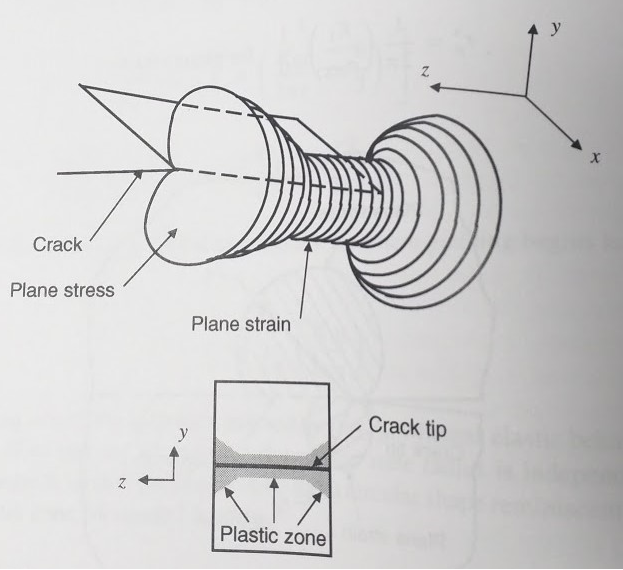
\includegraphics{../images/dumbell.png}
\caption{An image showing the 3D plastic zone shape, which looks a
little bit like a dumbell. The plastic zone is much larger near the
surface, where the material behaves as if in plane stress. In the
center, where the material behaves more like plane strain, the plastic
zone is much smaller.}
\end{figure}
\end{frame}

\begin{frame}{example}
\protect\hypertarget{example-3}{}
online example \href{../examples/Plastic\%20Zone\%20Shape.html}{here}
\end{frame}

\hypertarget{group-problems}{%
\section{group problems}\label{group-problems}}

\begin{frame}{group one}
\protect\hypertarget{group-one}{}
\begin{itemize}
\tightlist
\item
  Calculate the plastic zone size for an infinitely wide, center-cracked
  panel
\item
  Consider a crack-length of 4 cm, and a yield strength of
  \(\sigma_{YS}=55 \text{ MPa}\), with an applied load of
  \(\sigma = 20 \text{ MPa}\)
\item
  Assume the panel is very thin
\end{itemize}
\end{frame}

\begin{frame}{group two}
\protect\hypertarget{group-two}{}
\begin{itemize}
\tightlist
\item
  Calculate the plastic zone size for an infinitely wide, center-cracked
  panel
\item
  Consider a crack-length of 4 cm, and a yield strength of
  \(\sigma_{YS}=55 \text{ MPa}\), with an applied load of
  \(\sigma = 20 \text{ MPa}\)
\item
  Assume the panel is very thick
\end{itemize}
\end{frame}

\begin{frame}{group three}
\protect\hypertarget{group-three}{}
\begin{itemize}
\tightlist
\item
  Calculate the plastic zone size for an infinitely wide, center-cracked
  panel
\item
  Consider a crack-length of 4 cm, and a yield strength of
  \(\sigma_{YS}=55 \text{ MPa}\), with an applied load of
  \(\sigma = 20 \text{ MPa}\)
\item
  The panel thickness is \emph{t} = 0.65 cm
\end{itemize}
\end{frame}

\begin{frame}{group four}
\protect\hypertarget{group-four}{}
\begin{itemize}
\tightlist
\item
  Find the plastic stress intensity ratio for an infinitely wide,
  center-cracked panel
\item
  What factors will increase or decrease the plastic stress intensity
  ratio?
\end{itemize}
\end{frame}

\end{document}
